\documentclass[border=10pt]{standalone}
\usepackage[left=25mm,right=25mm,top=25mm,bottom=25mm]{geometry}
\usepackage[utf8]{inputenc}
\usepackage[T1]{fontenc}
\usepackage{times}
\usepackage{geometry}
\usepackage{amsmath}
\usepackage{amssymb}
\usepackage{mathrsfs}
\usepackage{amsfonts}
\usepackage{amsthm}
\usepackage{lipsum}
\usepackage{amscd}
\usepackage{graphicx}
\usepackage{fancyhdr}
\usepackage{textcomp}
\usepackage{txfonts}
\usepackage[all]{xy}
\usepackage{paralist}
\usepackage[colorlinks=true]{hyperref}
\usepackage{array}
\usepackage{tikz}
\usepackage{slashed}
\usepackage{pdfpages}
\usepackage{cite}
\usepackage{url}
\usepackage{amsmath,amsfonts,amssymb}
\usepackage{tikz}
\usetikzlibrary{arrows,matrix,positioning}
\usetikzlibrary{overlay-beamer-styles}
\usetikzlibrary{matrix.skeleton}
\usetikzlibrary{automata,positioning}
\usepackage{listings}
\usepackage{multirow}
\usepackage{color}

\begin{document}

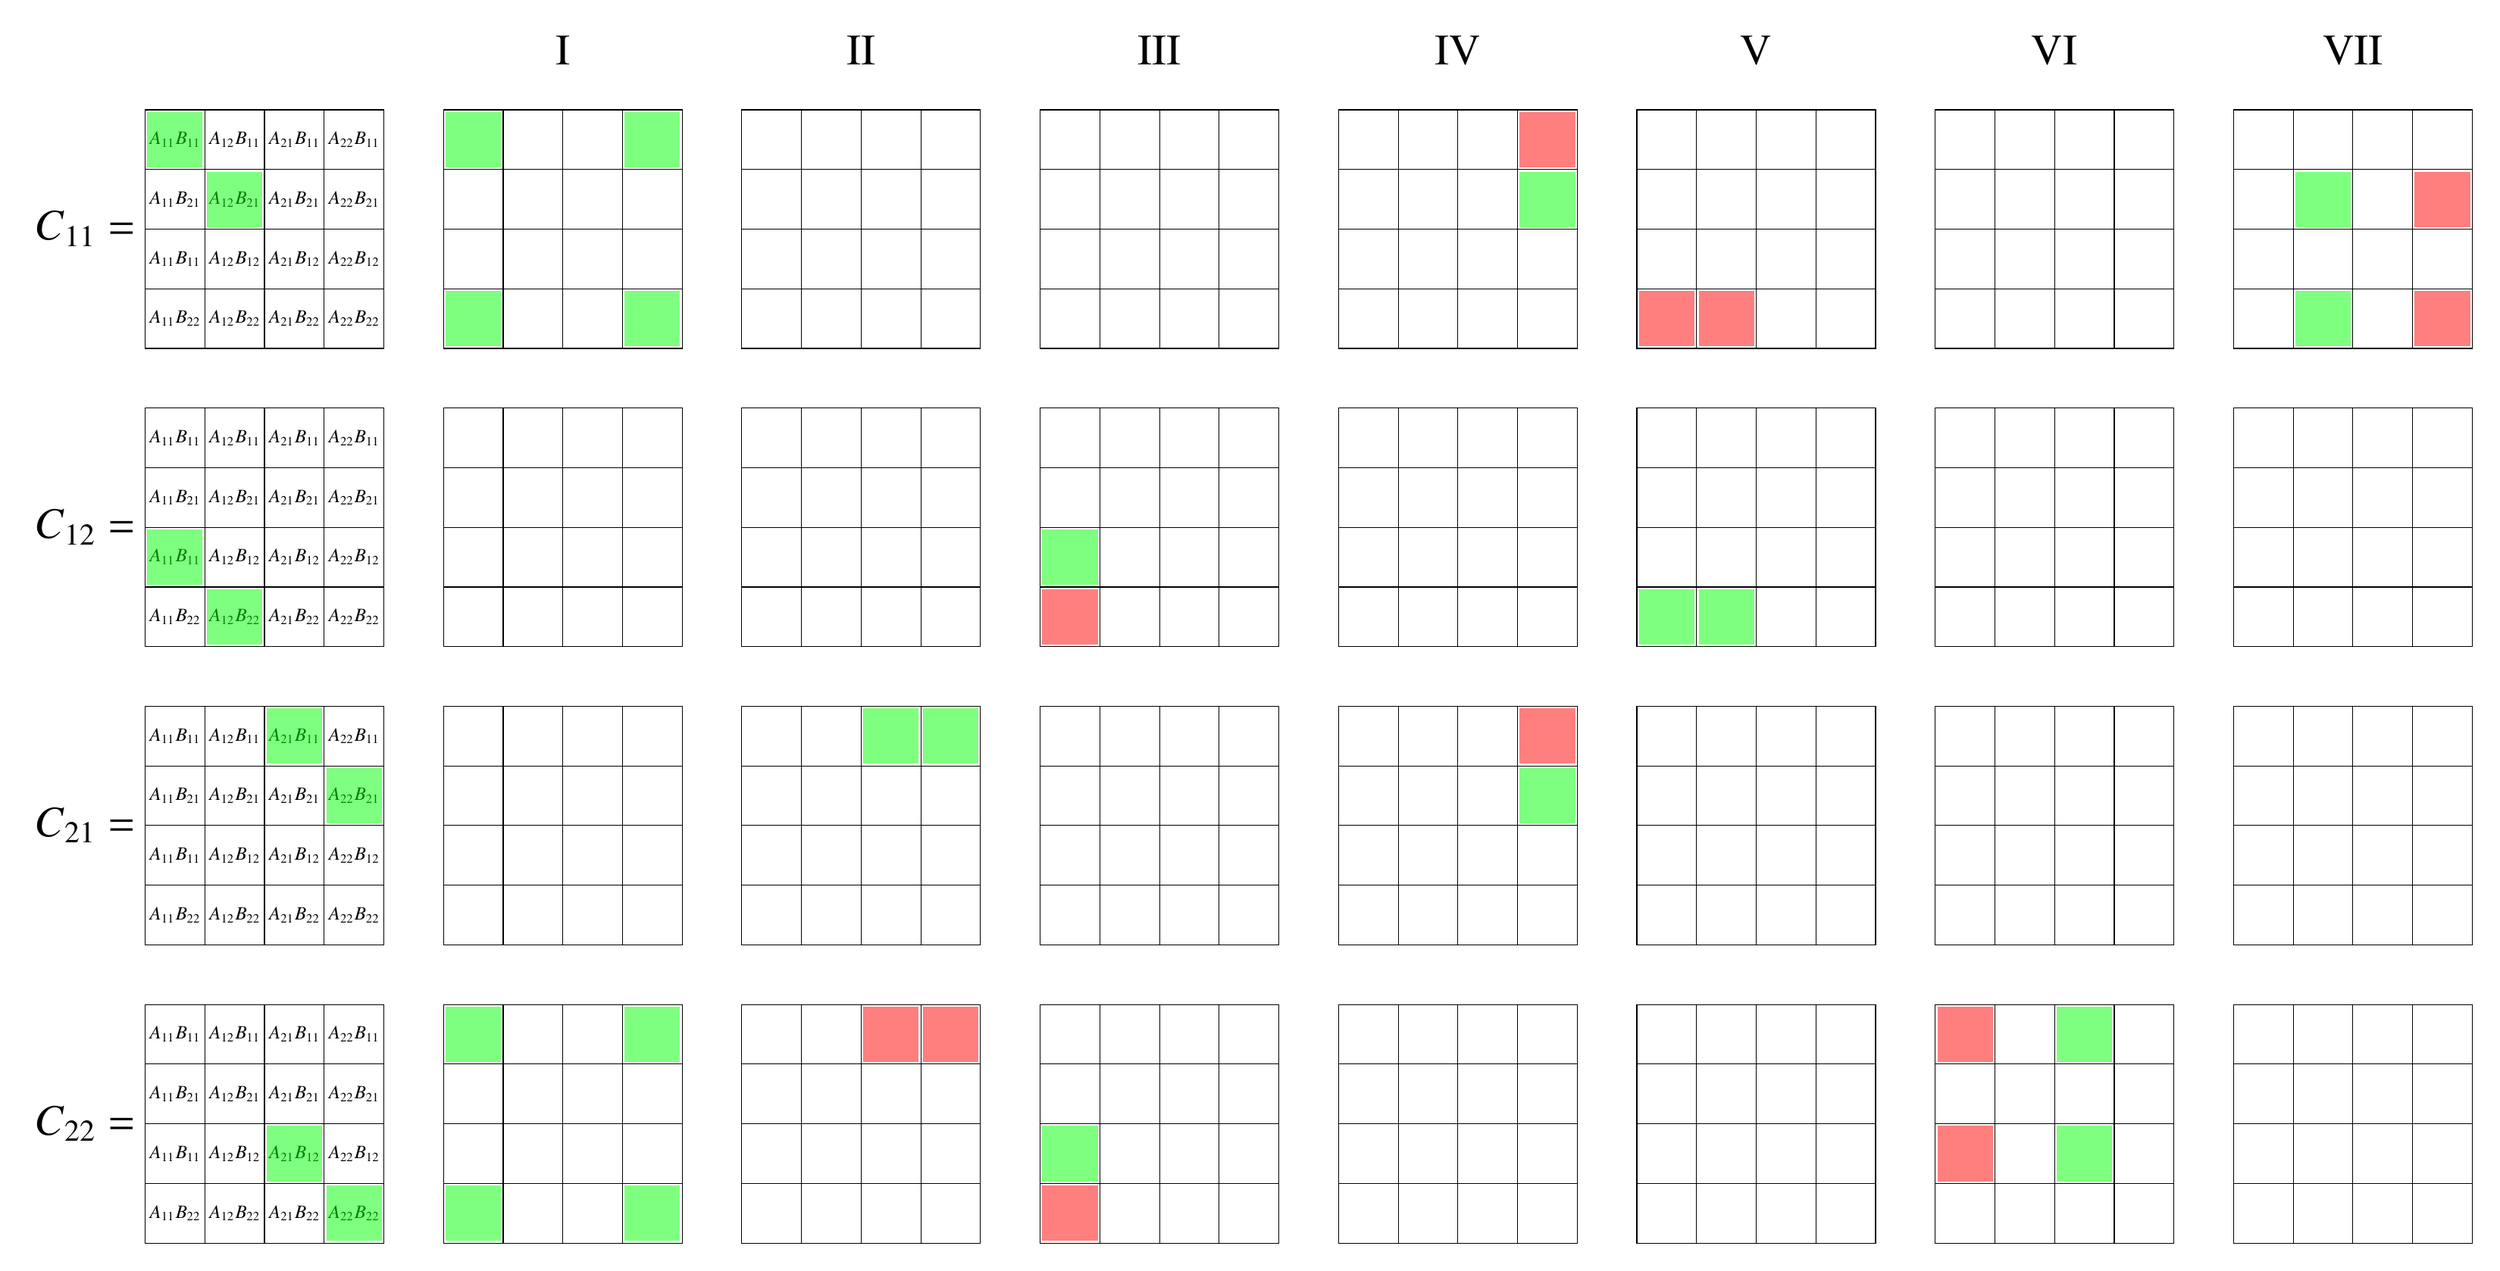
\begin{tikzpicture}[ampersand replacement=\&]

  \foreach \i in {1,...,4}
  {
  \small{
    \matrix (X\i)[matrix of math nodes,nodes in empty cells,
              nodes = {draw, minimum size=10mm,
                       anchor=center,
                       inner sep=0pt, outer sep=0pt},
              column sep=-\pgflinewidth,
              row sep=-\pgflinewidth,
              ] at (0,-\i*5)
   {
   A_{11}B_{11} \& A_{12}B_{11} \& A_{21}B_{11} \& A_{22}B_{11} \\
   A_{11}B_{21} \& A_{12}B_{21} \& A_{21}B_{21} \& A_{22}B_{21} \\
   A_{11}B_{11} \& A_{12}B_{12} \& A_{21}B_{12} \& A_{22}B_{12} \\
   A_{11}B_{22} \& A_{12}B_{22} \& A_{21}B_{22} \& A_{22}B_{22} \\
   };}

    \foreach \j in {1,...,7}
    {
    \matrix(M\i\j)[matrix of math nodes,nodes in empty cells,
                nodes = {draw, minimum size=10mm,
                         anchor=center,
                         inner sep=0pt, outer sep=0pt},
                column sep=-\pgflinewidth,
                row sep=-\pgflinewidth,
                ] at (\j*5,-\i*5)
     {
     \& \& \& \\
     \& \& \& \\
     \& \& \& \\
     \& \& \& \\
     };
   }
 }

\huge{
 \node at (-3,-20)  {$C_{22}=$};
 \node at (-3,-15) {$C_{21}=$} ;
 \node at (-3,-10) {$C_{12}=$} ;
 \node at (-3,-5) {$C_{11}=$} ;

 \node at (5,-2)  {I};
 \node at (10,-2)  {II};
 \node at (15,-2)  {III};
 \node at (20,-2)  {IV};
 \node at (25,-2)  {V};
 \node at (30,-2)  {VI};
 \node at (35,-2)  {VII};
 }


 \node[opacity=0.5, rounded corners=0pt, inner sep=-1pt, fill=green, fit=(X1-1-1)] {};
 \node[opacity=0.5, rounded corners=0pt, inner sep=-1pt, fill=green, fit=(X1-2-2)] {};
 \node[opacity=0.5, rounded corners=0pt, inner sep=-1pt, fill=green, fit=(X2-3-1)] {};
 \node[opacity=0.5, rounded corners=0pt, inner sep=-1pt, fill=green, fit=(X2-4-2)] {};
 \node[opacity=0.5, rounded corners=0pt, inner sep=-1pt, fill=green, fit=(X3-1-3)] {};
 \node[opacity=0.5, rounded corners=0pt, inner sep=-1pt, fill=green, fit=(X3-2-4)] {};
 \node[opacity=0.5, rounded corners=0pt, inner sep=-1pt, fill=green, fit=(X4-3-3)] {};
 \node[opacity=0.5, rounded corners=0pt, inner sep=-1pt, fill=green, fit=(X4-4-4)] {};

 \node[opacity=0.5, rounded corners=0pt, inner sep=-1pt, fill=green, fit=(M11-4-1)] {};
 \node[opacity=0.5, rounded corners=0pt, inner sep=-1pt, fill=green, fit=(M11-1-4)] {};
 \node[opacity=0.5, rounded corners=0pt, inner sep=-1pt, fill=green, fit=(M11-4-4)] {};
 \node[opacity=0.5, rounded corners=0pt, inner sep=-1pt, fill=green, fit=(M11-1-1)] {};
 \node[opacity=0.5, rounded corners=0pt, inner sep=-1pt, fill=red, fit=(M14-1-4)] {};
 \node[opacity=0.5, rounded corners=0pt, inner sep=-1pt, fill=green, fit=(M14-2-4)] {};
 \node[opacity=0.5, rounded corners=0pt, inner sep=-1pt, fill=red, fit=(M15-4-1)] {};
 \node[opacity=0.5, rounded corners=0pt, inner sep=-1pt, fill=red, fit=(M15-4-2)] {};
 \node[opacity=0.5, rounded corners=0pt, inner sep=-1pt, fill=red, fit=(M17-2-4)] {};
 \node[opacity=0.5, rounded corners=0pt, inner sep=-1pt, fill=red, fit=(M17-4-4)] {};
 \node[opacity=0.5, rounded corners=0pt, inner sep=-1pt, fill=green, fit=(M17-2-2)] {};
 \node[opacity=0.5, rounded corners=0pt, inner sep=-1pt, fill=green, fit=(M17-4-2)] {};

 \node[opacity=0.5, rounded corners=0pt, inner sep=-1pt, fill=green, fit=(M23-3-1)] {};
 \node[opacity=0.5, rounded corners=0pt, inner sep=-1pt, fill=red, fit=(M23-4-1)] {};
 \node[opacity=0.5, rounded corners=0pt, inner sep=-1pt, fill=green, fit=(M25-4-1)] {};
 \node[opacity=0.5, rounded corners=0pt, inner sep=-1pt, fill=green, fit=(M25-4-2)] {};

 \node[opacity=0.5, rounded corners=0pt, inner sep=-1pt, fill=green, fit=(M32-1-4)] {};
 \node[opacity=0.5, rounded corners=0pt, inner sep=-1pt, fill=green, fit=(M32-1-3)] {};
 \node[opacity=0.5, rounded corners=0pt, inner sep=-1pt, fill=red, fit=(M34-1-4)] {};
 \node[opacity=0.5, rounded corners=0pt, inner sep=-1pt, fill=green, fit=(M34-2-4)] {};

 \node[opacity=0.5, rounded corners=0pt, inner sep=-1pt, fill=green, fit=(M41-4-1)] {};
 \node[opacity=0.5, rounded corners=0pt, inner sep=-1pt, fill=green, fit=(M41-1-4)] {};
 \node[opacity=0.5, rounded corners=0pt, inner sep=-1pt, fill=green, fit=(M41-4-4)] {};
 \node[opacity=0.5, rounded corners=0pt, inner sep=-1pt, fill=green, fit=(M41-1-1)] {};
 \node[opacity=0.5, rounded corners=0pt, inner sep=-1pt, fill=red, fit=(M42-1-4)] {};
 \node[opacity=0.5, rounded corners=0pt, inner sep=-1pt, fill=red, fit=(M42-1-3)] {};
 \node[opacity=0.5, rounded corners=0pt, inner sep=-1pt, fill=green, fit=(M43-3-1)] {};
 \node[opacity=0.5, rounded corners=0pt, inner sep=-1pt, fill=red, fit=(M43-4-1)] {};
 \node[opacity=0.5, rounded corners=0pt, inner sep=-1pt, fill=green, fit=(M46-1-3)] {};
 \node[opacity=0.5, rounded corners=0pt, inner sep=-1pt, fill=red, fit=(M46-1-1)] {};
 \node[opacity=0.5, rounded corners=0pt, inner sep=-1pt, fill=green, fit=(M46-3-3)] {};
 \node[opacity=0.5, rounded corners=0pt, inner sep=-1pt, fill=red, fit=(M46-3-1)] {};
\end{tikzpicture}



\end{document}
